% \documentclass{article}
\documentclass[12pt]{beamer}
\usepackage{biblatex} %Imports biblatex package
\usepackage{booktabs}
% \usepackage{minipage}
\addbibresource{bibliography.bib} %Import the bibliography file
\usepackage[orientation=landscape,size=a0,scale=0.8]{beamerposter}
\usepackage{graphicx}
\usepackage[font=small]{subcaption} % Required for inserting images
\setbeamertemplate{caption}[numbered]
\usecolortheme{orchid}
\setbeamerfont{block title}{series=\bfseries, size=\huge}
\setbeamerfont{title}{series=\bfseries,  size=\Huge}
\setbeamerfont{author}{ size=\large}
\setbeamerfont{institute}{ size=\large}
\setbeamerfont{date}{ size=\large}

% \setbeamerfont{block body}{size=\small}
\title{Automatic Identification of Giant Kelp Reproductive Features with Deep Learning}
\logo{
\includegraphics[height=2\baselineskip]{uwm logo}}
\title{%
  \texorpdfstring{%
    \makebox[\linewidth]{%
      \makebox[0pt][l]{%
        \raisebox{\dimexpr-\height+\baselineskip}[0pt][0pt]
          {\hspace{4em}
\includegraphics[height=2\baselineskip]{uwm logo}}% Left logo, bit inelegant
      }\hfill
      \makebox[0pt]{Automatic Identification of Giant Kelp Reproductive Features with Deep Learning}%
      \hfill\makebox[0pt][r]{%
        \raisebox{\dimexpr-\height+\baselineskip}[0pt][0pt]{}
          % {\includegraphics[height=2\baselineskip]{example-image-b}}% Right logo
      }%
    }%
  }
  {Automatic Identification of Giant Kelp Reproductive Features with Deep Learning}} % Poster title

\author{Liam Jemison}
\date{\today}
\institute{University of Wisconsin Milwaukee}
% \logo{
\includegraphics[height=4cm]{uwm logo}}
% \usetheme{Simple}
% \renewcommand*{\bibfont}{\scriptsize}

\begin{document}


% \begin{columns}
%     \column{0.3}
\begin{frame}{}
\setbeamercolor{section in sidebar}{fg=structure.fg!20!white}
\setbeamercolor{subsection in sidebar}{fg=structure.fg!20!white}
\maketitle
\begin{columns}[t]
      \begin{column}{.30\linewidth}

      
        \begin{block}{Introduction}
            \vspace{1em}
          Algae are frequently stored in the gametophyte stage in the laboratory. This is more efficient than storing large plants, and gametophytes can be maintained in low-light and low-temperature environments essentially indefinitely.

          \begin{figure}%[Trays of gametophytes (left), gametophytes at 100x magnification (right)]
                \centering
                \begin{subfigure}{0.49\linewidth}
                     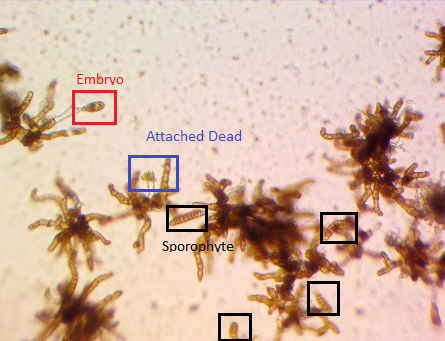
\includegraphics[width=\linewidth]{annotated kelp.png}
                \end{subfigure} \hfill
                \begin{subfigure}{0.49\linewidth}
                     % \subfloat[\centering Giant Kelp gametophytes at 100x magnification]{}%
                     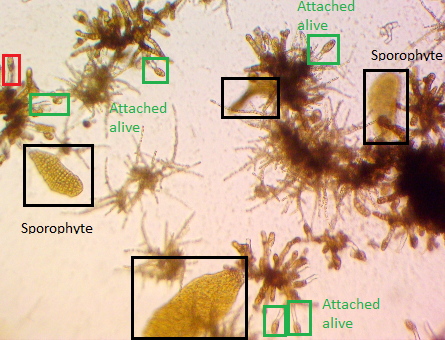
\includegraphics[width=\linewidth]{annotated kelp 2.png}
                \end{subfigure}
               \caption{Example features of interest}\label{features}
               \end{figure}

          
          However, gathering even rudimentary data on the tiny gametophytes is time consuming, requiring manual inspection of cultures, which may number in the dozens or hundreds, under a microscope. To streamline the process of acquiring this data, we train Yolo-X object detection networks to identify \emph{Macrocystis} and \emph{Nereocystis} reproductive structures at 100x magnification, along the way producing a novel dataset of annotated sporophyte features. We show that through \emph{tiling} the same network can identify features at a variety of magnifications
        \end{block}
        \begin{block}{Reproductive Features dataset}
        We constructed a new dataset of more than 1000 images of kelp gametophytes captured at 100x magnification on a mu-1000 amscope camera, taken throughout the early sporophyte stage, containing 3,422 labeled objects. In Figure \ref{subfig:class-counts} we show the breakdown of instances by class. 
        \vspace{1em}
            \begin{figure}
\centering
    \begin{subfigure}{0.49\linewidth}
         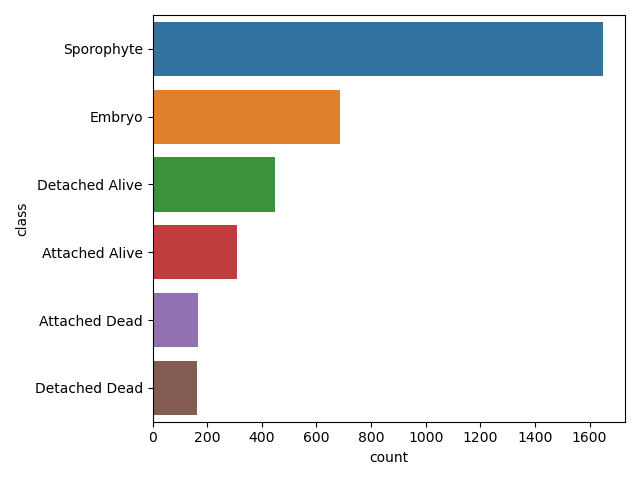
\includegraphics[width=\linewidth]{counts}
         \subcaption{Class counts.}\label{subfig:class-counts}
    \end{subfigure} \hfill
    \begin{subfigure}{0.42\linewidth}
         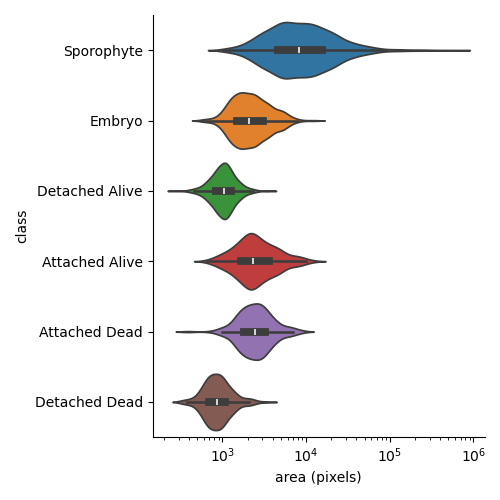
\includegraphics[width=\linewidth]{sizes}
    \subcaption{Distribution of bounding  box areas.}
    \end{subfigure}
\caption{Left: number of annotations created of each of the categories.  Right: distribution of area of bounding box annotations.} \label{fig:dataset-statistics}
\end{figure}
        In Figure \ref{features} we show examples of the reproductive features of interest. Especially in the early stages of development, it can be challenging to pick out sporophytes from the normal gametophyte structure. 
        \end{block}
      \end{column}

      
      \begin{column}{.30\linewidth}
       \begin{block}{Object Detection}
                \vspace{1em}
                
             In the field of computer vision, object detection generally refers to the task of classifying and drawing a bounding box around, or segmenting, pixels of interest in static images. In recent years, deep neural network object detectors have achieved excellent performance on bounding box detection when trained on large datasets \cite{lin_microsoft_2015} and increasingly on segmentation as well. Extending these results to smaller datasets and datasets with large numbers of unusual objects is still an active area of research \cite{gupta_lvis_2019}. Object detectors have been applied to a variety of ecological applications, including camera traps \cite{schneider_deep_2018, noauthor_cameratrapsmegadetectormd_nodate, norouzzadeh_deep_2021}, cell microscopy \cite{waithe_object_2020, hung_applying_2019}, and tracking fish populations \cite{lopez-marcano_automatic_2021, ditria_automating_2020}.
        
             Even state-of-the-art object detectors struggle with occluded objects, objects classes with significant variation in size, and crowds of similar objects \cite{zhan2022trilayer, hutchison_diagnosing_2012}, making the identification of kelp reproductive structures a challenging task. Our annotators attempt to label all reproductive structures, even those which are out of focus, obscured or partially truncated but the labelling process is nonetheless subjective. 
        \end{block}
        \begin{block}{Methods}
            \vspace{1em}
            %this part describes the actual training set up and should be modified depending on what I wind up going with there. 
            Using the {\tt mmdetection} \cite{chen_mmdetection_2019} library, we trained several variations of the YOLOX\cite{ge_yolox_2021} object detection network. By varying the number of parameters in the network, we can observe the trade-off in inference speed and network performance. This approach also produces several models which support different hardware configurations in the end use. Training is conducted on a single Nvidia RTX 3090 graphics card. 
            
            Before training, we randomly separate 20\% of the total dataset for validation. We train for 600 epochs, validating every 10 epochs. After training, we keep the weights with the greatest mean average precision at 0.5 confidence. We perform moderate augmentation, including flipping, resizing, padding, random color transforms, mixup and mosaic augmentation.  . We do not attempt to optimize hyperparameters, instead using a configuration that is very similar to the {\tt mmdetection} yolo-x-coco configuration.

            For a demonstration of the network, you can visit \url{https://huggingface.co/spaces/liam-jemison/kelp}
        \end{block}
    \begin{block}{Results}
    \vspace{1em}
            We follow the standard practice of validating our detection models against annotated data that was held out from the training process. We compare the inferences of the detection models against the annotations created by a human annotator. A prediction is associated to a particular ground truth annotation if the intersection of the the predicted and true boxes, divided by the union of the predicted and true boxes, (IoU) is above some threshold. Following the COCO evaluation protocol\cite{lin_microsoft_2015}, we report the average precision (AP) of each model at different IoU thresholds in Figure \ref{ap-fps}. 
     For our large model, we show classification metrics by class in Figure \ref{classification-metric}, with IoU threshold of 0.1 and confidence level 0.5. 
     \vspace{1em}
     \begin{figure}
     \begin{subfigure}[b]{0.49\linewidth}
                 % \centering
         \begin{tabular}{lrrrr}
            \toprule
            {} &  precision &  recall &  f1-score &  support \\
            category       &            &         &           &          \\
            \midrule
            Attached\_Alive &       0.52 &    0.42 &      0.47 &    59.00 \\
            Attached\_Dead  &       0.67 &    0.36 &      0.47 &    39.00 \\
            Detached\_Alive &       0.70 &    0.86 &      0.77 &    69.00 \\
            Detached\_Dead  &       0.72 &    0.50 &      0.59 &    26.00 \\
            Embryon        &       0.70 &    0.62 &      0.66 &   145.00 \\
            Sporophyte     &       0.85 &    0.86 &      0.86 &   368.00 \\
            micro avg      &       0.77 &    0.73 &      0.75 &   706.00 \\
            macro avg      &       0.69 &    0.60 &      0.63 &   706.00 \\
            weighted avg   &       0.76 &    0.73 &      0.74 &   706.00 \\
            \bottomrule
        \end{tabular}
        \caption{Classification metrics of large Yolo-X model}\label{classification-metric}
     \end{subfigure}\hfill
     \begin{subfigure}[b]{0.5\linewidth}
        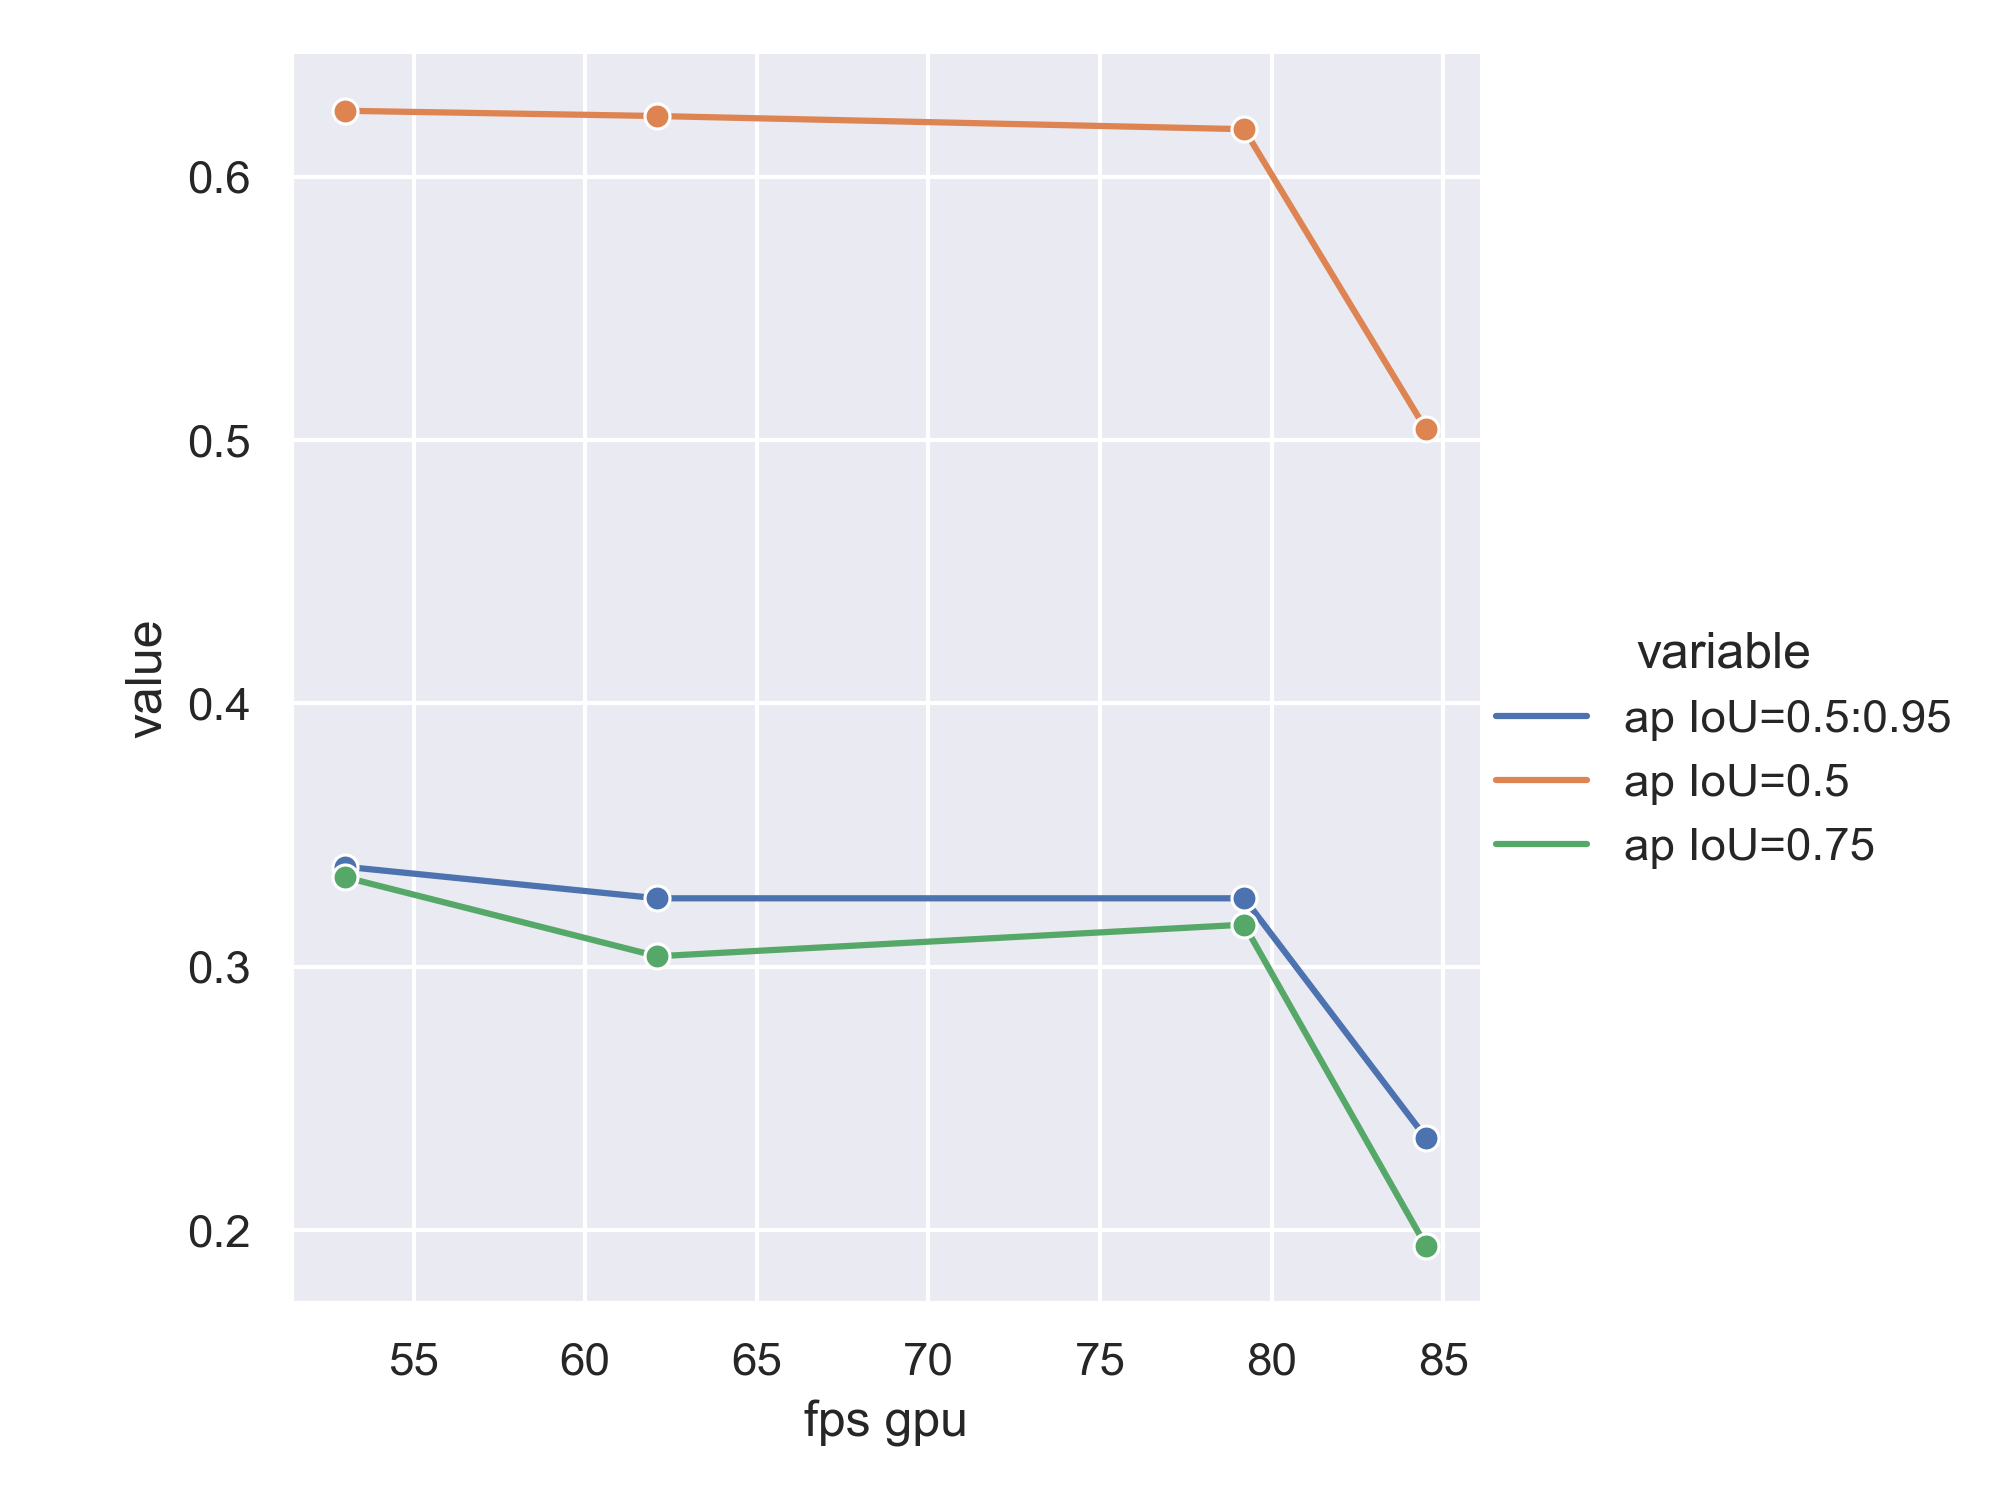
\includegraphics{ap vs fps}
          \caption{Average Precision and inference speed (fps) of object detection networks}\label{ap-fps}
     \end{subfigure}
     \caption{Network performance}\label{classification}
     \end{figure}
    In Figure \ref{worst} we show the two images with the greatest number of false positives from the validation set. As expected, these are crowded scenes with occluded objects. In clear scenes with little occlusion and crowding, model performance is generally good
     \begin{figure}
                \centering
                \begin{subfigure}{0.49\linewidth}
                    %\subfloat[\centering Trays of kelp gametophytes]
                    {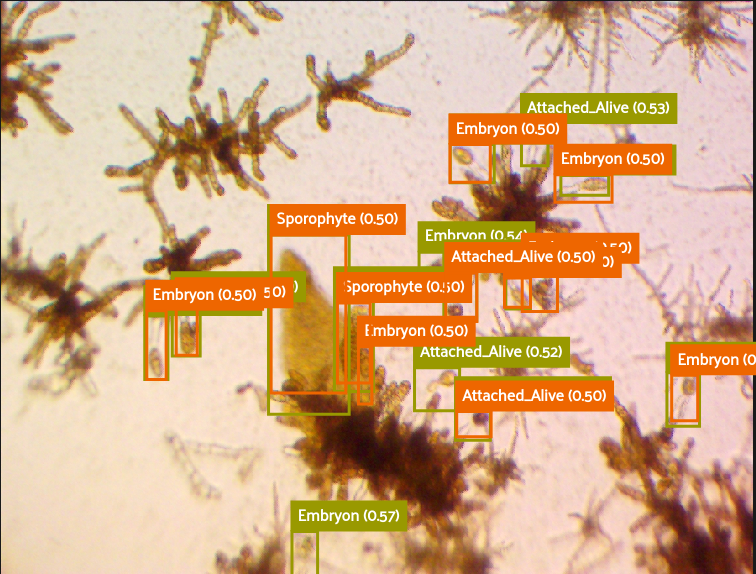
\includegraphics[width=\linewidth]{worst detection.png}}
                    % \caption{Network inference without tiling}
                \end{subfigure} \hfill
                \begin{subfigure}{0.49\linewidth}
                     % \subfloat[\centering Giant Kelp gametophytes at 100x magnification]{}%
                     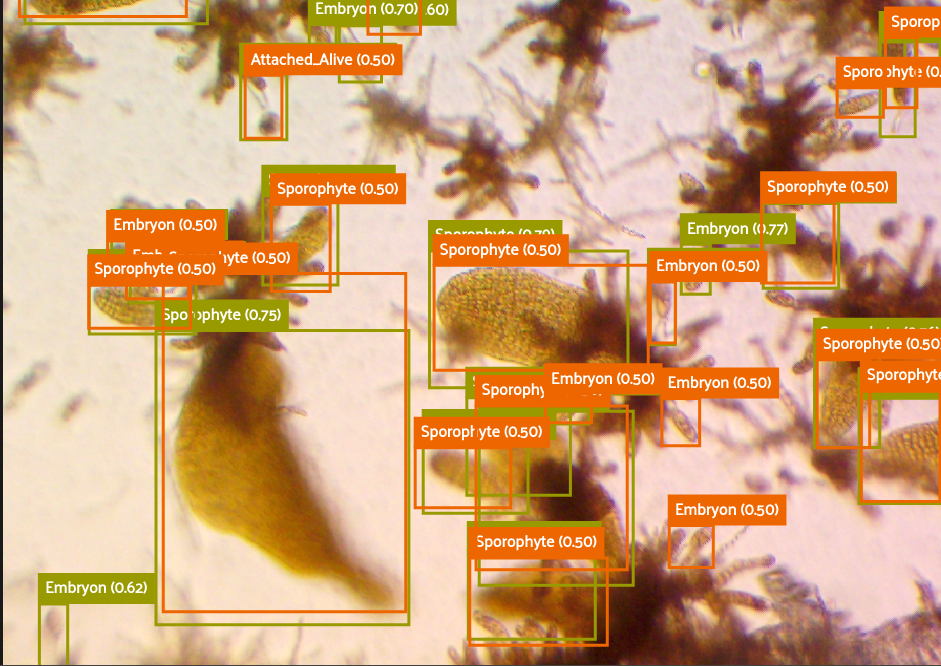
\includegraphics[width=\linewidth]{worst detection 2.png} 
                     % \caption{Network inference with tiling}
                \end{subfigure}
               
                     \caption{Images with greatest number of false positive predictions from validation set. Ground truth labels are orange, green labels are predictions.}\label{worst}
            \end{figure}
    \end{block}
      \end{column}
      \begin{column}{.30\linewidth}
        \begin{block}{Tiling}
        \vspace{1em}
            Because our dataset of reproductive features consists of images captured at 100x magnification, the models we created struggle to identify objects in images taken at different magnifications. However this issue can be ameliorated by tiling input images into a series of smaller images. For example, to identify objects in an image taken at 40x magnification, one may crop the original image into four smaller images, each of which will roughly match the scale of the training images. In Figure \ref{tiling} you can see that the network correctly identifies 7 sporophytes with no tiling, and 13 sporophytes with tiling, out of a total of 16, significantly better performance. 
            \begin{figure}
                \centering
                \begin{subfigure}{0.49\linewidth}
                    {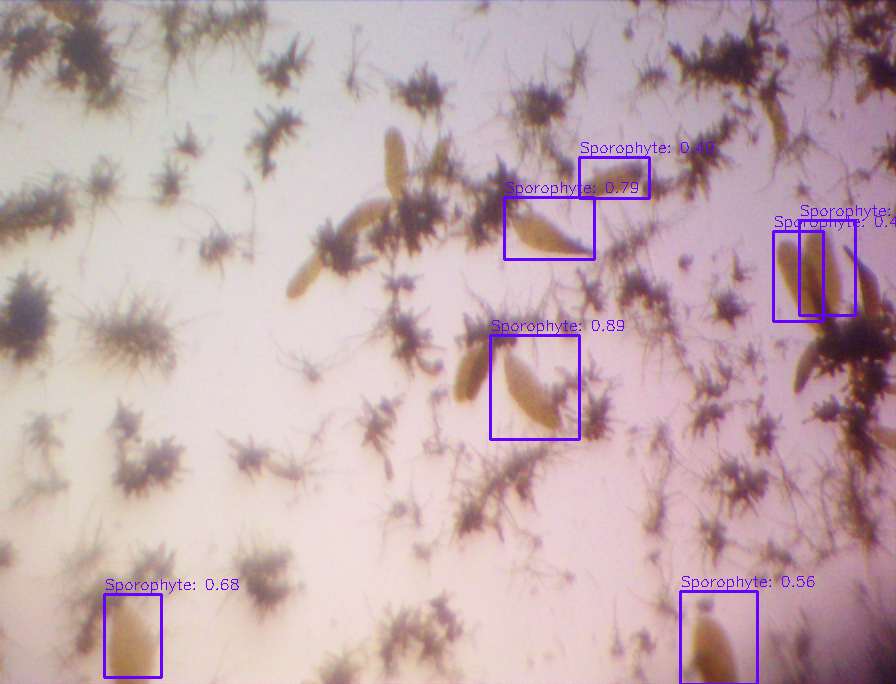
\includegraphics[width=\linewidth]{100x_no_tiling}}
                    \caption{Network inference without tiling}
                \end{subfigure} \hfill
                \begin{subfigure}{0.49\linewidth}
                     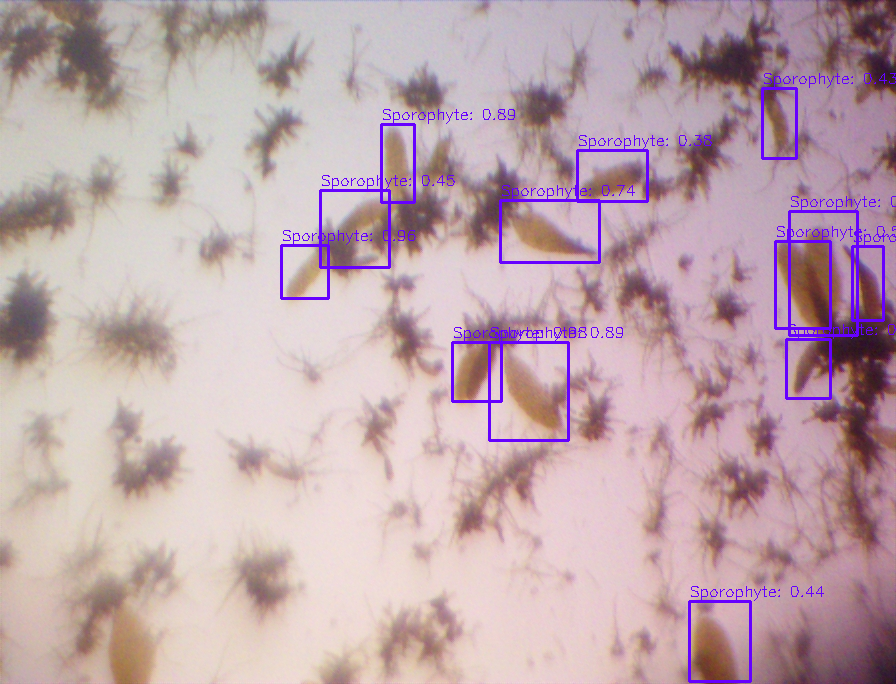
\includegraphics[width=\linewidth]{100x_tiling} 
                     \caption{Network inference with tiling}
                \end{subfigure}
                     \caption{Application of tiling to 40x magnfication image}\label{tiling}
            \end{figure}
            \end{block}
            

          \begin{block}{References}
          \vspace{1em}
            \printbibliography
              
          \end{block}
      \end{column}
    \end{columns}
\end{frame}
\end{document}
